\documentclass[a4paper,12pt]{article}
\usepackage{amsmath}
\usepackage{bm}
\usepackage[mathscr]{euscript}
\usepackage{graphicx}
\graphicspath{ {images/} }
\begin{document}

\title{Additional Comments on our Code}

\author{Marcel Dürr \and Enes Witwit}

\section{Introduction}

In this document, we will recapitulate our code and provide further explanations on selected excerpts of our code

\section{Mesh}

We start of with our mesh generator 'mesh\_generate'. Our domain $\Omega = [0,1]^2$ will not be subject to change for this task, therefore our only input will be the mesh size $h$. The result will be two matrices, namely \textit{vertex\_matrix} and \textit{cell\_matrix}. \textit{vertex\_matrix} will store the coordinates of each vertex, while \textit{cell\_matrix} only stores the numbers of the four vertices of each cell.
\\
\textit{Example}: $h=0.5$

\[\mbox{\textit{vertex\_matrix}}=\begin{pmatrix} 0&0\\0.5&0\\1&0\\0&0.5\\0.5&0.5\\1&0.5\\0&1\\0.5&1\\1&1\\\end{pmatrix},\ \mbox{\textit{cell\_matrix}}=\begin{pmatrix} 1&2&4&5\\2&3&5&6\\4&5&7&8\\5&6&8&9\\
\end{pmatrix}\]

\section{Shape Functions}

An essential concept for finite element methods would be shape functions. We have to set up certain points, so called \textit{nodes} on a reference cell $\hat T = [0,1]^2$ such that our shape functions $p_i$ are uniquely defined by two properties: 
\begin{enumerate}
\item $p_i(x_j)=\delta_{ij}, \ x_j \mbox{node}$
\item $p_i$ is a polynomial on each edge.
\end{enumerate} 
A way to achieve this, is to choose the location of the nodes in the same way as our mesh. Afterwards, we choose appropriate base-polynomials. If we want polynomials of degree $k$ on the edges, the appropriate basis would be $\{x^iy^j, \ i,j=0...k\}$. Although the resulting polynomials are of order $2k$, they are only of order $k$ in each variable and therefore only of order $k$ on each edge. A mesh generated with mesh-size $\frac{1}{k}$ will yield $k+1$ nodes on each edge; the interpolation is well-posed. \\
\textit{Remark}: The way we order our basis has to be consistent for the entire code, because we only store the coefficients when we want to store a polynomial. In particular, this means that one entry of the coefficient vector must refer to the same polynomial basis element, even for different orders of polynomials. Effectively, this means that the basis for a higher order polynomial can only add basis elements at the end of any lower order polynomial basis. \\
\\
\textit{sf\_generate} follows this scheme closely. Since the shape functions only depend on the polynomial degree $k$ we want to have on the edges, our only input will be the integer $k$. The function will create the nodes using \textit{mesh\_generate} with mesh-size $\frac{1}{k}$. Next, it will create a data-set, containing the coordinates and the value at these coordinates for each node. In total, we get $(k+1)^2:=n$ nodes, their values are computed using the Kronecker Delta. This will ensure, that property 1) holds true when interpolating over all these points. The interpolation is done by solving
\[\begin{pmatrix} 1 &\ x_0 &\ \cdots &\ x_0^ky_0^k \\
\vdots &\ \vdots &\ \ddots &\ \vdots \\ 
1 &\ x_{n} &\ \cdots &\ x_{n}^ky_{n}^k \end{pmatrix}
\begin{pmatrix} a_0 \\ \vdots \\ a_n \end{pmatrix}=\begin{pmatrix} b_0 \\ \vdots \\ b_n \end{pmatrix}\]
The output of our function is the matrix $SF$, which stores the coefficient vectors of each shape function in its rows. Again, we see that a consistent numbering is needed when we want to evaluate a shape function. Let's look at some shape functions:\\
\textit{Example}: Let the polynomial degree on the edges be 1. The coefficient matrix \textit{SF} will look like this:\\
\[\begin{pmatrix}
1&-1&-1&1\\0&1&0&-1\\0&0&1&-1\\0&0&0&1\
\end{pmatrix}\\\]
\newpage
The four resulting shape functions:\\
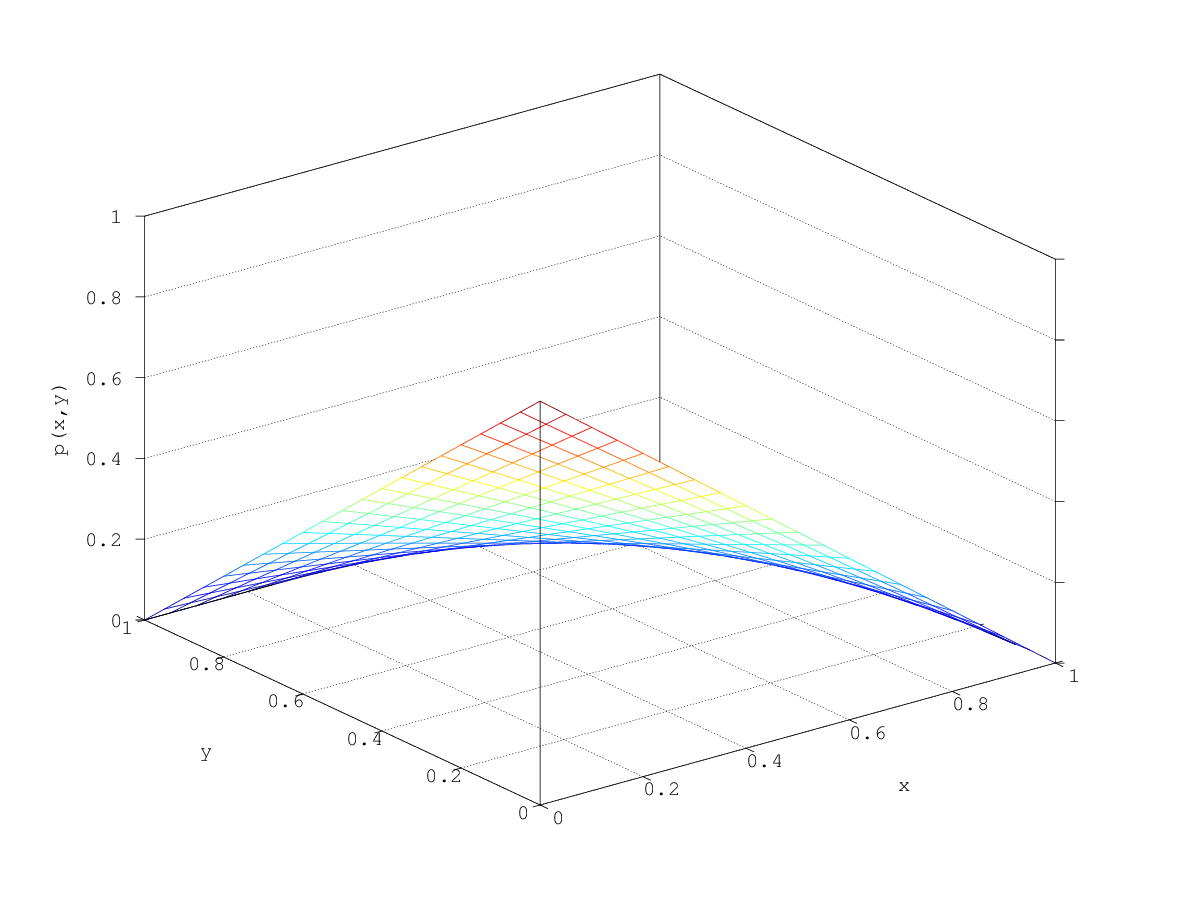
\includegraphics[scale=0.35]{P1} 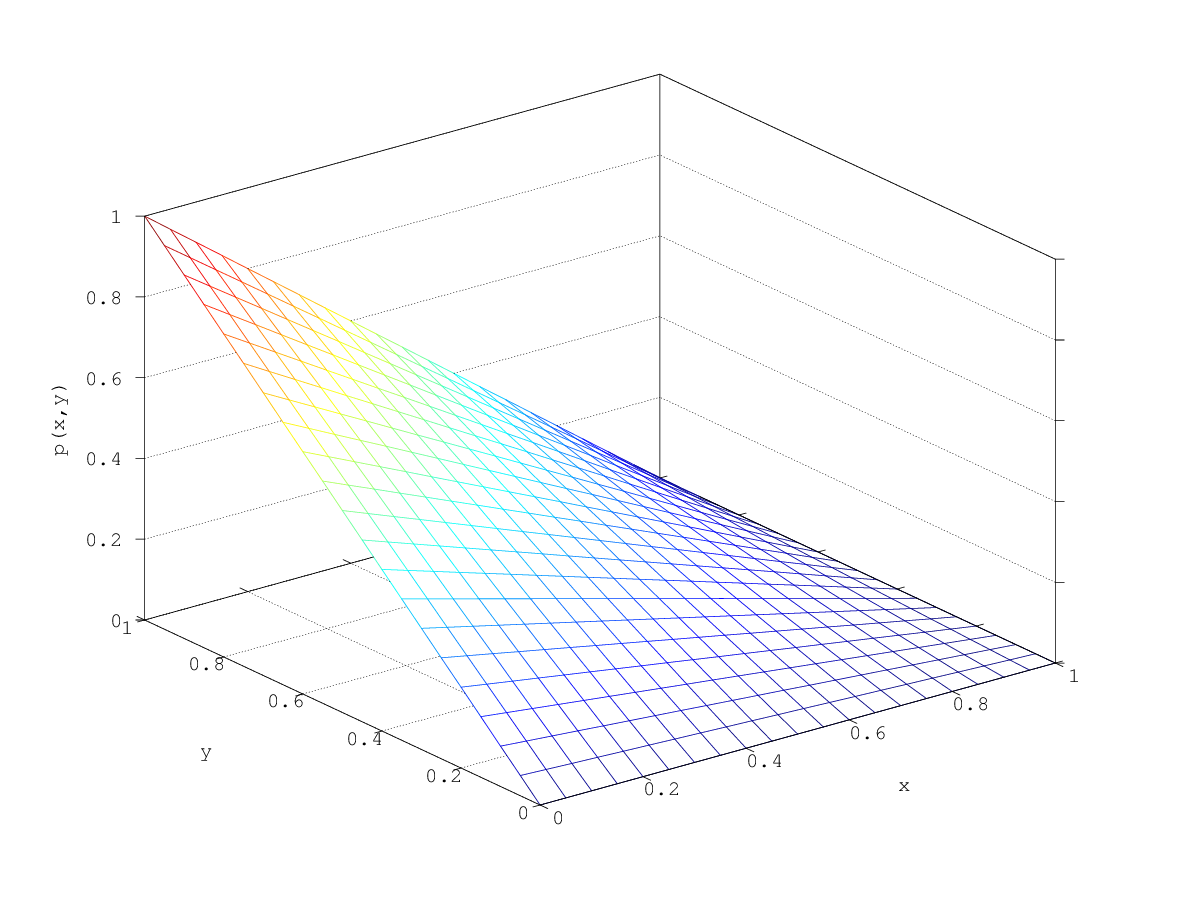
\includegraphics[scale=0.35]{P2} 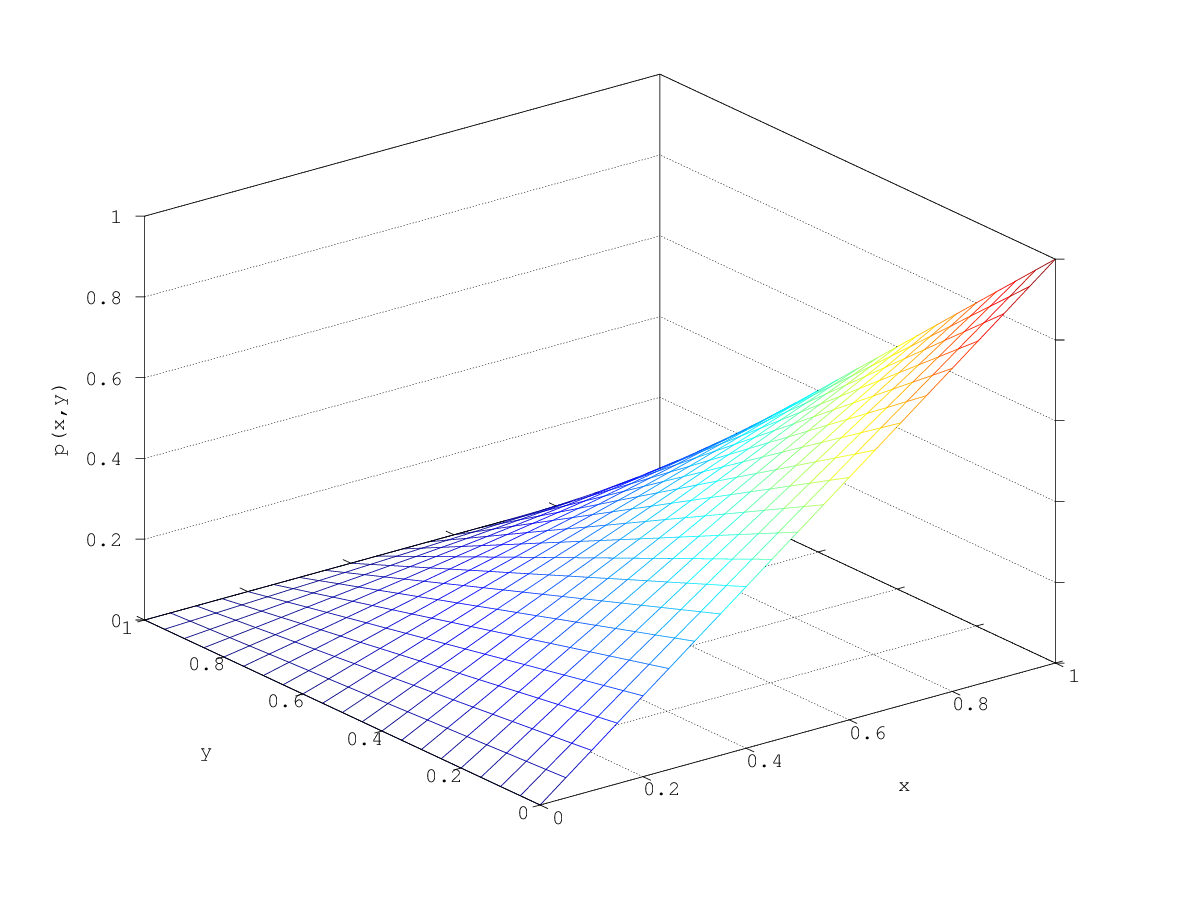
\includegraphics[scale=0.35]{P3} 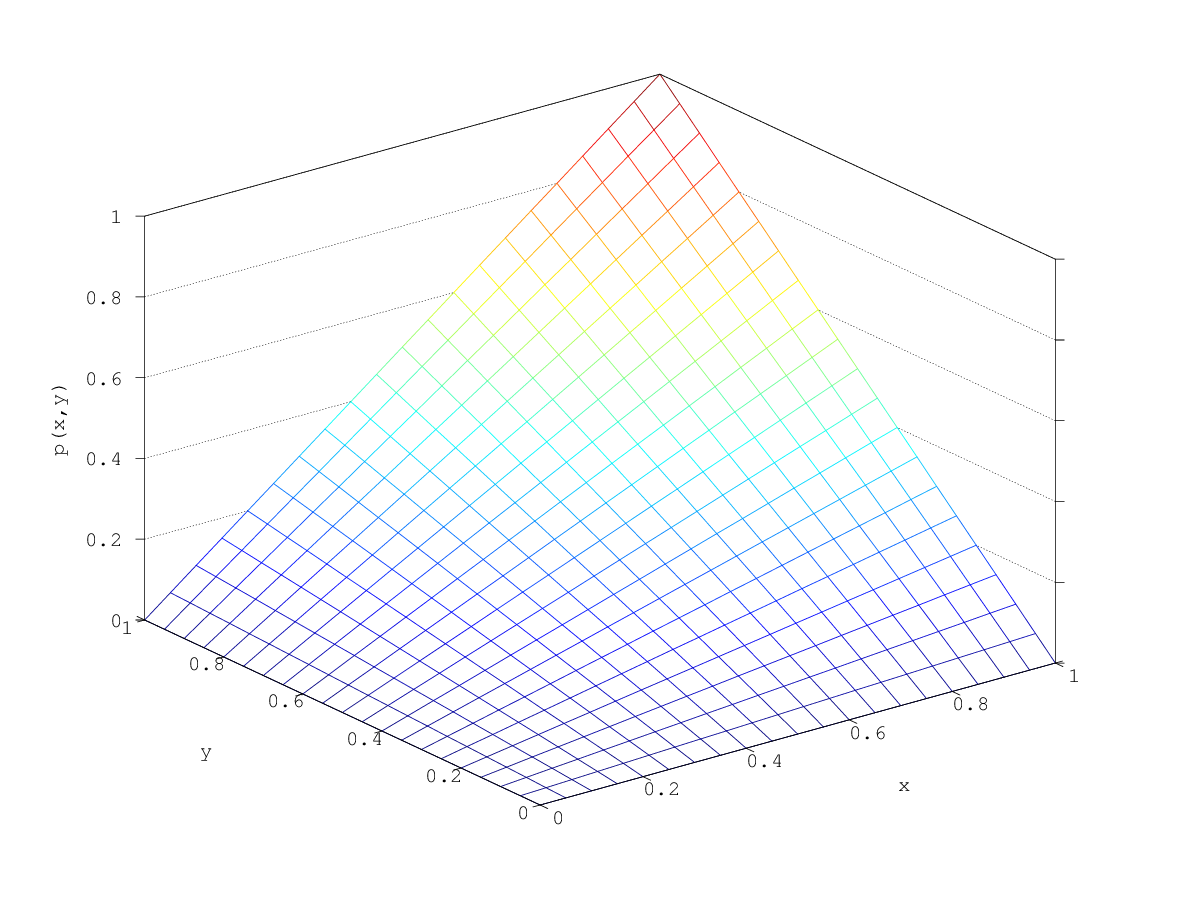
\includegraphics[scale=0.35]{P4}
You can clearly see, that each shape function has the value 1 at one vertex, and 0 at all the other vertices
\section{Stiffness Matrix}
Next up is the assembly of the stiffness matrix, this will be the left hand side of our linear system. The original idea behind the stiffness matrix was to build every combination of our basis functions in our bilinear form, namely $A_{ij}=a(\phi_i,\phi_j)$. As seen in the lecture, it is more efficient to compute a \textit{local} stiffness matrix for each cell, and then insert these values in the right way in a global stiffness matrix. This approach proves to be even more efficient, considering that in our case, the local stiffness matrices are identical for each cell (\textit{see also}: Theoretical Construct, Chapter 'Integrals and Transformations').\\
\\
The computation of the local matrix is done by \textit{sm\_assemble\_local}. As already shown, the computation will not depend on a specific cell, therefore we only need the mesh-size $h$ and the shape function coefficients $SF$. Furthermore, we need several help functions which will compute the required integrals
\begin{itemize}
\item \textit{hf\_eval\_poly} will evaluate a given polynomal at a given point, by using our specific polynomial basis and a coefficient vector
\item \textit{sf\_derivate} will return the coefficient vectors for the derivative in x and y direction for a given polynomial. 
\item \textit{int\_gauss\_weights} will return quadrature points and weigths for a given order and a given quadratic domain.
\item \textit{int\_gauss} will evaluate a given function at the quadrature points and sum over the product of the quadrature weigths. 
\end{itemize} 
Note that the computation of the quadrature points and the actual quadrature is split up into two function. The transformations we use enable us to only integrate over the unit square. Therefore, we only have to compute the quadrature points and weights once. This will save alot of recources.\\
Having these functions at hand, the local matrix can be easily computed. The symmetric bilinear form will result in a symmetric local matrix, we will only compute on half if the matrix.\\
\\
The next step will be the assembly of the global stiffness matrix.
Let $(a_{ij})^T$ be the local stiffness matrix for a cell $T$. For any given $i$ and $j$, the entry in the global stiffness matrix can be obtained by \[A_{ij}=\sum_{T \in \mathscr{T}_h}a_{\rho^{-1}(i)\rho(j)^{-1}}^T\] where $\rho$ will map the local node numbering to the global numbering. The most efficient way to implement this, is to iterate over all cells, and add the entries of the local matrix at the right spot.\\
\\
Key to this operation is the mapping $\rho$. Our function \textit{mesh\_nodes} will handle the renumbering by generating a matrix. The $i$-th row corresponds to the $i$-th cell, the $j$-th entry in this row corresponds to the $j$-th local node within the cell. In this entry, the matrix will store the global number of the degree of freedom, which corresponds to the $j$-th local node of the $i$-th cell. For each iteration, we will select the corresponding entries of the global matrix by using \textit{mesh\_nodes} and simply add the local stiffness matrix.

\section{Right Hand Side}
The linear system is still missing its right hand side. We already discussed the computation of it in the 'Theoretical Construct', Chapter 'Integrals and Transformations'. The function \textit{rhs\_integration} will compute the right hand side. \\
This function works in a similar fashion to the assembly of the global stiffness matrix. Given a cell, this function will integrate over every shape function at once, the function \textit{mesh\_nodes} will add the resulting vector at the correct spot. We use octave's build-in function \textit{repmat} to multiplay our rigth hand side $f$ to every entry of \textit{hf\_eval\_poly}. 
\section{Linear Solvers}
The global stiffness matrix will be sparse, due to the way we chose the basis functions (zero on the vast majority of the cells). The prefered solvers for linear systems with sparse matrices are iterative solvers. We implemented two common algorithms, namely the \textit{generalized minimal residual method} and the \textit{conjugate gradient method}. 
We are left with a coefficient vector $u$. We will get our solution, by building the linear combination of the basis ${\phi_i}$ with $u$: 
\[u_h = \sum \phi_i u_i\]
Remember, that we do not actually have the basis functions $\phi_i$ at hand, since we accessed the needed values by using shape functions and transforming the integral. We will need an auxiliary function to evaluate $u_h$

\section{Evaluation of the Solution}
The idea behind \textit{hf\_eval\_solution} is to find the indices of the basis functions, that do not vanish at a given point $(x,y)$. Similar to the calculation of the right hand side, we will need to know which shape function should be evaluated at which cell. Additionally, we need to know to which entry of the coefficient vector $u$ the computation correlates.\\
In the special case, that $(x,y)$ lies on a node, the function will return the corresponding entry of $u_h$.If not, \textit{hf\_eval\_solution} starts searching for adjacent cells to the given point $(x,y)$, at which we want to evaluate our solution. Once we have the numbers of the active cells, we want to know, which nodes are located on these cells. We will store the local and the global number of the node. This leaves us with a matrix with rows consisting of the local node number, the corresponding global node number and the cell, on which the node lies. If a node lies on an edge between two cells, only one cell will be stored, the other one will be ommited. It remains to evaluate the correct shapefunction over the correct cell and multiply with the corresponding entry of $u_h$.

\section{Presentation our Results}
Our function \textit{m\_plot\_solution} will create three plots:
\begin{itemize}
\item The analytical solution
\item The right hand side of the strong formulation (to show, that it is a multiple of the solution)
\item The approximation, using \textit{hf\_eval\_solution} and the coefficient vector $u_h$
\end{itemize}

blabla ParaView blabla

\section{Error analysis}

\section{Appendix}
This section will highlight some function, that were programmed in a very specific way to suit our needs. Since matrix and vector operations are optimized in Octave, we avoided for-loops with many iterations and tried utilizing matrix or vector operations.\\ \\
\textit{Evaluation of a Polynomial}\\ \\
Normaly, you would want to evaluate a polynomial $p$ only at a single point $(x,y)\in\!R$. For our problem, it will be benificial to multiple polynomials at once. We designed \textit{hf\_eval\_poly} in a way, that we can have the whole coefficient matrix $SF$ as an input, and therefore get a vector with a value for each shape function as an output. To utilize Octave's full potential, we also wanted to be able to have two matrices as inputs, instead of only single points. This will create a matrix, containing a column of blockmatrices. Each blockmatrix will resemble one shape function, evaluated at the given set of points by the two matrices.\\ \\
\newpage
\textit{Gauss Quadrature}\\ \\
Given the sample points $(x_1,...,x_n)^T$ and weights $(w_1,...,w_n)^T$, the gauss quadrature of a function $f$ in 2-D is given by
\[\sum_{i,j} w_i w_j f(x_i,x_j)\]
Instead of using for-loops, we use Octave's build-in function \textit{meshgrid} to create rank one matrices $W_1,W_2$ for the weigths $w_i$ and $X,Y$ for sample points $x_i$. Evaluating $f(X,Y)$ will create the matrix 
\[\begin{pmatrix} f(x_1,x_1) &\ f(x_1,x_2) &\ \cdots &\ f(x_1,x_n) \\
\vdots &\ \vdots &\ \ddots &\ \vdots \\ 
f(x_n,x_1) &\ f(x_n,x_2) &\ \cdots &\ f(x_n,x_n) \end{pmatrix} \]
Using component-wise multiplication, we get 
\[\begin{pmatrix} w_1 w_ 1f(x_1,x_1) &\ w_1 w_2 f(x_1,x_2) &\ \cdots &\ w_1 w_n f(x_1,x_n) \\
\vdots &\ \vdots &\ \ddots &\ \vdots \\ 
w_n w_1 f(x_n,x_1) &\ w_n w_2 f(x_n,x_2) &\ \cdots &\ w_n w_n f(x_n,x_n) \end{pmatrix} \]
Adding all entries of the matrix will give the desired quadrature. Our function \textit{int\_gauss\_vectorized} does exactly this. The function will fail when confronted with vector or even matrix-valued functions. We had to write a more complex function \textit{int\_gauss\_vectorized\_matrices}, that has the ability to sum over submatrices, and return the correct quadrature for every component. We will explain this function with an example:\\
Let $f$ be a matrix-valued function
\begin{equation}f(x,y)=\begin{pmatrix} f_{1 1}(x,y) &\ f_{1 2}(x,y) \\
						 f_{2 1}(x,y) &\ f_{2 2}(x,y) \\
                         f_{3 1}(x,y) &\ f_{3 2}(x,y) \end{pmatrix}
\end{equation}
Using Octave's \textit{repmat} function, we can obtain a matrix, consisting of submatrices,
\[M=\begin{pmatrix} A &\ B \\
			      C &\ D \\
                  E &\ F \end{pmatrix}\]

Where each submatrix has the form of (1). Let $A,B,C,D,E,F \in \!R^{3\times 3}$ for this example. We will generate two matrices and multiply them to the matrix $M$:
\[\begin{pmatrix} \begin{pmatrix} A_{1 1} &\ A_{1 2} &\ A_{1 3}\\
						 A_{2 1} &\ A_{2 2} &\ A_{2 3}\\
                         A_{3 1} &\ A_{3 2} &\ A_{3 3}\end{pmatrix} &\ \begin{pmatrix} B_{1 1} &\ B_{1 2} &\ B_{1 3}\\
						 B_{2 1} &\ B_{2 2} &\ B_{2 3}\\
                         B_{3 1} &\ B_{3 2} &\ B_{3 3}\end{pmatrix} \\ \begin{pmatrix} C_{1 1} &\ C_{1 2} &\ C_{1 3}\\
						 C_{2 1} &\ C_{2 2} &\ C_{2 3}\\
                         C_{3 1} &\ C_{3 2} &\ C_{3 3}\end{pmatrix} &\ \begin{pmatrix} D_{1 1} &\ D_{1 2} &\ D_{1 3}\\
						 D_{2 1} &\ D_{2 2} &\ D_{2 3}\\
                         D_{3 1} &\ D_{3 2} &\ D_{3 3}\end{pmatrix} \\ \begin{pmatrix} E_{1 1} &\ E_{1 2} &\ E_{1 3}\\
						 E_{2 1} &\ E_{2 2} &\ E_{2 3}\\
                         E_{3 1} &\ E_{3 2} &\ E_{3 3}\end{pmatrix} &\ \begin{pmatrix} F_{1 1} &\ F_{1 2} &\ F_{1 3}\\
						 F_{2 1} &\ F_{2 2} &\ F_{2 3}\\
                         F_{3 1} &\ F_{3 2} &\ F_{3 3}\end{pmatrix} \end{pmatrix} \begin{pmatrix} 1 &\ 0 \\ 1 &\ 0 \\ 1 &\ 0 \\0 &\ 1 \\ 0 &\ 1 \\ 0 &\ 1 \end{pmatrix} = 
\begin{pmatrix} \bar{A_1} &\ \bar{B_1} \\ \bar{A_2} &\ \bar{B_2} \\\bar{A_3} &\ \bar{B_3} \\\bar{C_1} &\ \bar{D_1} \\\bar{C_2} &\ \bar{D_2} \\\bar{C_3} &\ \bar{D_3} \\\bar{E_1} &\ \bar{F_1} \\\bar{E_2} &\ \bar{F_2} \\\bar{E_3} &\ \bar{F_3} \\ \end{pmatrix} \]

Where $\bar{A_i}$ is the sum of the entries of the $i$-th row of $A$. We can now transpose this matrix and multiply with another auxiliary matrix

\[\begin{pmatrix} \bar{A_1} &\ \bar{A_2} &\ \bar{A_3} &\ \bar{C_1} &\ \bar{C_2} &\ \bar{C_3} &\ \bar{E_1} &\ \bar{E_2} &\ \bar{E_3} \\
\bar{B_1} &\ \bar{B_2} &\ \bar{B_3} &\ \bar{D_1} &\ \bar{D_2} &\ \bar{D_3} &\ \bar{F_1} &\ \bar{F_2} &\ \bar{F_3} \end{pmatrix}
\begin{pmatrix} 1 &\ 0 &\ 0 \\
				1 &\ 0 &\ 0 \\
                1 &\ 0 &\ 0 \\
                0 &\ 1 &\ 0 \\
                0 &\ 1 &\ 0 \\
                0 &\ 1 &\ 0 \\
                0 &\ 0 &\ 1 \\
                0 &\ 0 &\ 1 \\
                0 &\ 0 &\ 1 \end{pmatrix} = \begin{pmatrix} A^* &\ C^* &\ E^* \\ B^* &\ D^* &\ F^* \end{pmatrix} \]
Where $A^*$ is the desired sum of the submatrix $A$. Transposing this matrix yields the succesfull quadrature.
\end{document}
